\documentclass[]{beamer}
%for printing or having a crappy pdf reader backup
%\documentclass[handout]{beamer}
\mode<presentation>
\usetheme{Madrid}


\usecolortheme[RGB={80,0,0}]{structure}
%teal \usecolortheme[RGB={0,128,128}]{structure}
\useoutertheme{miniframes}
\useinnertheme{default}
\usepackage{color}
\definecolor{Maroon}{RGB}{80,0,0}
\definecolor{BurntOrange}{RGB}{204,85,0}
\usepackage{setspace}
\usepackage{amsmath}
\usepackage{amsthm}
\usepackage{amsfonts}
\usepackage{amssymb}
\usepackage{verbatim}
\usepackage{array}
\usepackage{graphicx}
\usepackage{subfigure}
\usepackage{colortbl}
\usepackage[retainorgcmds]{IEEEtrantools}
\usepackage{wrapfig}
\usepackage[figurename=,tablename=]{caption}
\usepackage{multirow}
\setbeamercolor{normal text}{fg=black}
\setbeamercovered{dynamic}
\beamertemplatetransparentcovereddynamicmedium
%\usepackage{chronology}
\setbeamertemplate{caption}[numbered]


\newcommand {\mathsym}[1]{{}}
\newcommand {\unicode}{{}}
\newcommand{\om}{\boldsymbol{\Omega}}
\newcommand{\etal}{{\it et al.\,}}
\newcommand{\vr}{\vec{r}}
\newcommand{\vo}{\vec{\Omega}}
\newcolumntype{L}{>{\centering\arraybackslash}m{3cm}}
\newcommand{\tcr}[1]{\textcolor{red}{#1}}
%Creating a norm command
\newcommand{\norm}[1]{\left\lVert#1\right\rVert}
%Allow page breaks within align
\allowdisplaybreaks
%Code
\usepackage{listings}
\newlength \figwidth
\setlength \figwidth {0.5\textwidth}


\begin{document}
%	

\title[Load Balancing]{Load Balancing Unstructured Meshes for Massively Parallel Transport Sweeps}
\author[Ghaddar]{Tarek Ghaddar \\ Chair: Dr. Jean Ragusa \\ Committee: Dr. Jim Morel, Dr. Bojan Popov}
\institute[TAMU]{Texas A\&M University}
%\committee{Morel,Popov}{Dr. Jim Morel \\ Dr. Bojan Popov}
\date[March 8, 2016]

{
\setbeamertemplate{headline}[default] 
\begin{frame}
\vspace{-1.1cm}
	\begin{figure}[t]
		\centering
			
\includegraphics[width=.25\textwidth]{figures/seal.png}
	\end{figure}
\vspace{-0.75cm}
\titlepage
\end{frame}
}

\begin{frame}
\tableofcontents
\end{frame}

\section{Overview and Introduction}
\subsection{}
\begin{frame}[t]\frametitle{Motivation}
	\begin{block}{}
	\begin{itemize}
		\item When running any massively parallel code, load balancing is a priority in order to achieve the best possible parallel efficiency.
		\item  A load balanced problem has an equal number of degrees of freedom per processor.
		\item Load balancing a logically Cartesian mesh is not difficult, as the user specifies the number of cells being used.
		\item In an unstructured mesh, the user cannot always specify the number of cells they want per processor, and obtaining a load balanced problem is more difficult.
	\end{itemize}
	\end{block}
\end{frame}

\begin{frame}[t]\frametitle{PDT}
	\begin{block}{}
	\begin{itemize}
		\item All work presented in this thesis was implemented in Texas A\&M's massively parallel deterministic transport code, PDT. 
		\item It is capable of multi-group simulations and employs discrete ordinates for angular discretization.
		\item Features steady-state, time-dependent, criticality, and depletion simulations. It solves the transport equation for neutron, thermal, gamma, coupled neutron-gamma, electron, and coupled electron-photon radiation.
		\item  PDT  has been shown to scale on logically Cartesian grids out to 750,000 cores.
		\end{itemize}
	\end{block}
\end{frame}

\begin{frame}[t]\frametitle{The Triangle Mesh Generator}
	\begin{block}{}
	\begin{itemize}
		\item Unstructured meshes in PDT are generated using the Triangle Mesh Generator.
	\end{itemize}	
	\end{block}
	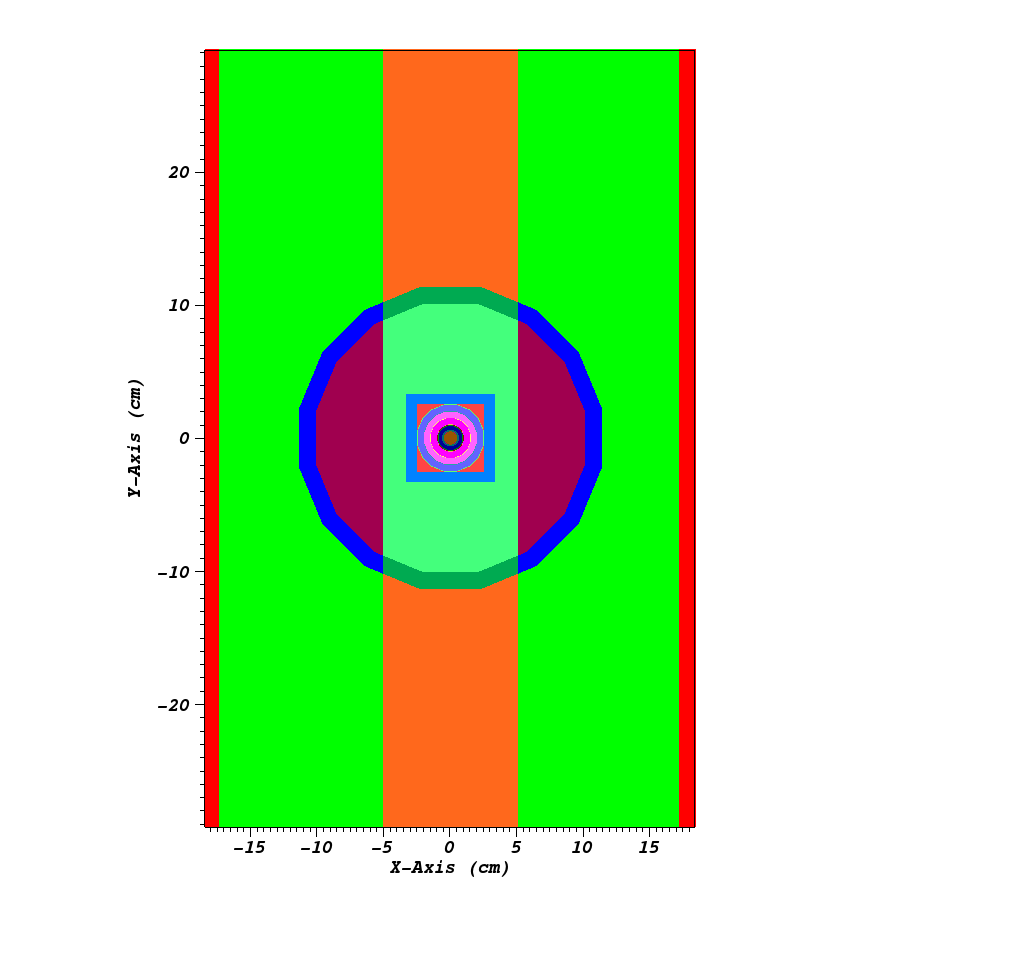
\includegraphics[scale = 0.15]{figures/IM12DPoly.png}
	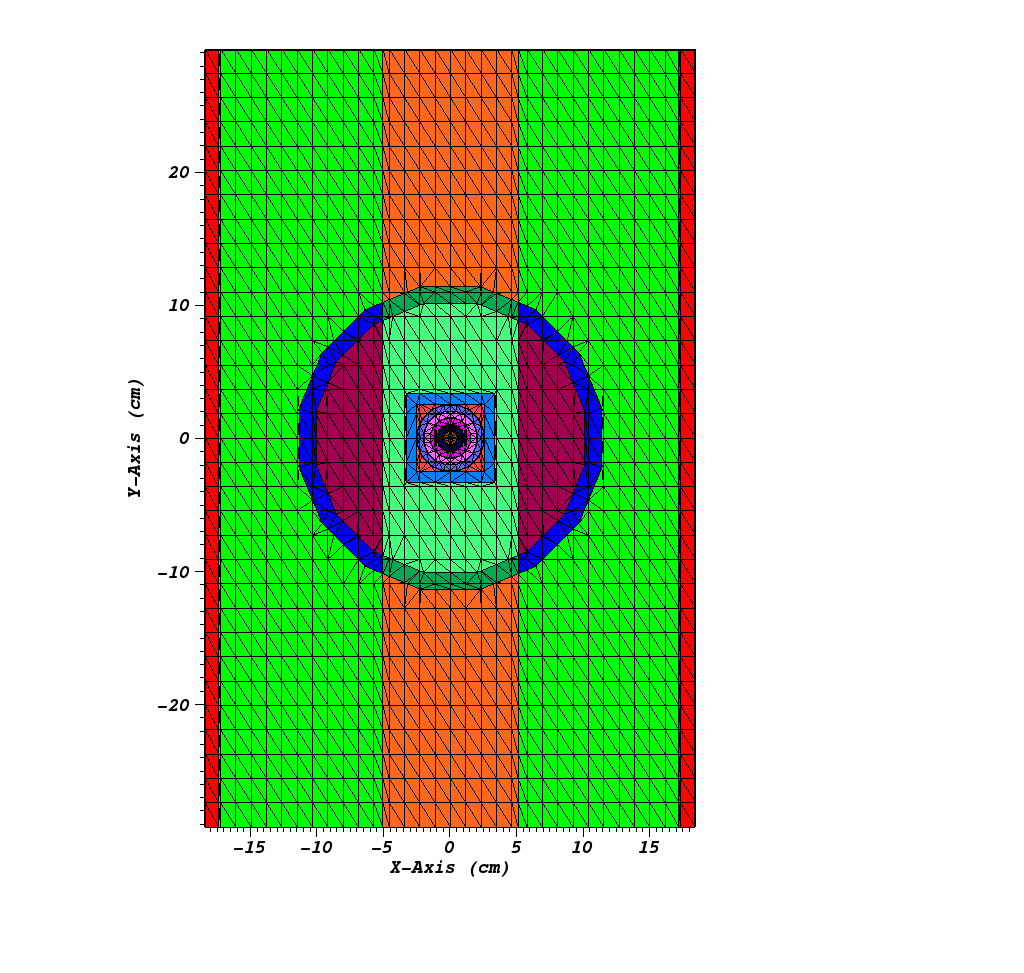
\includegraphics[scale = 0.15]{figures/IM12DMesh.png}
\end{frame}

%%The Transport Equation

\section{The Transport Equation}
\subsection{}
\begin{frame}[t]\frametitle{The Transport Equation}
	\begin{block}{}
	\begin{align*}
\hspace{-10cm} \vo \cdot \vec \nabla \psi(\vr,E,\vo) +\Sigma_t(\vr,E) \psi(\vr,E,\vo)  = \\ \int_{0}^{\infty}dE' \int_{4\pi}d\Omega' \Sigma_s(\vr,E'\to E, \Omega'\to\Omega)\psi(\vr,E',\vo') + S_{ext}(\vr,E,\vo)
	\label{continuous transport}
	\end{align*}
	\end{block}
	%\vspace{-0.3 cm}
	\begin{block}{}
	\begin{align*}
	\vo \cdot \vec \nabla \psi(\vr,E,\vo) +\Sigma_t(\vr,E) \psi(\vr,E,\vo)  
	= \\\frac{1}{4\pi}\int_{0}^{\infty}dE' \Sigma_s(\vr,E'\to E) \int_{4\pi}d\Omega' \psi(\vr,E',\vo')  + S_{ext}(\vr,E,\vo) \nonumber \\
	 = \frac{1}{4\pi}\int_{0}^{\infty}dE' \Sigma_s(\vr,E'\to E) \phi(\vr,E')  + S_{ext}(\vr,E,\vo)
	\end{align*}
	\end{block}
\end{frame}

\begin{frame}[t]\frametitle{The Transport Equation}
	\begin{block}{}
	\begin{align*}
		\phi(\vr,E') = \int_{4\pi}d\Omega' \psi(\vr,E',\vo')
	\end{align*}
	\end{block}
	\begin{block}{}
	\begin{align*}
	\vo \cdot \vec \nabla \psi_g(\vr,\vo) +\Sigma_{t,g}(\vr) \psi_g(\vr,\vo) = \frac{1}{4\pi}\sum_{g^{\prime}}\Sigma_{s,g^{\prime}\to g}(\vr)\phi_{g^{\prime}}(\vr) + S_{ext,g}(\vr,\vo), \\\quad \text{for } 1 \le g \le G
	\end{align*}
	\end{block}
\end{frame}

\begin{frame}[t]\frametitle{The Transport Equation}
	\begin{block}{}
	\begin{align*}
	\vo_m \cdot \vec \nabla \psi_{g,m}(\vr) +\Sigma_{t,g}(\vr) \psi_{g,m}(\vr)  = \frac{1}{4\pi}\sum_{g^{\prime}}\Sigma_{s,g^{\prime}\to g}(\vr)\phi_{g^{\prime}}(\vr) + S_{ext,g,m}(\vr)
	\end{align*}
	\end{block}
	\begin{block}{}
	\begin{align*}
	\phi_g(\vr) \approx \sum_{m=1}^{m=M} w_m \psi_{g,m}(\vr).
	\end{align*}
	\end{block}
	\begin{block}{}
	\begin{align*}
	\vo_m \cdot \vec\nabla \psi_m^{(l+1)}(\vr) + \Sigma_t \psi_m^{(l+1)}(\vr) = q_m^{(l)}(\vr)
	\end{align*}
	\end{block}
\end{frame}

\section{Parallel Transport Sweeps}
\subsection{}
\begin{frame}[t]\frametitle{The Transport Sweep}
	\begin{block}{}
	A parallel sweep algorithm is defined by three properties:
	\begin{itemize}
		\item partitioning: dividing the domain among available processors
		\item aggregation: grouping cells, directions, and energy groups into tasks
		\item scheduling: choosing which task to execute if more than one is available
	\end{itemize}
	\end{block}
	
\end{frame}

\begin{frame}[t]\frametitle{The Sweep}
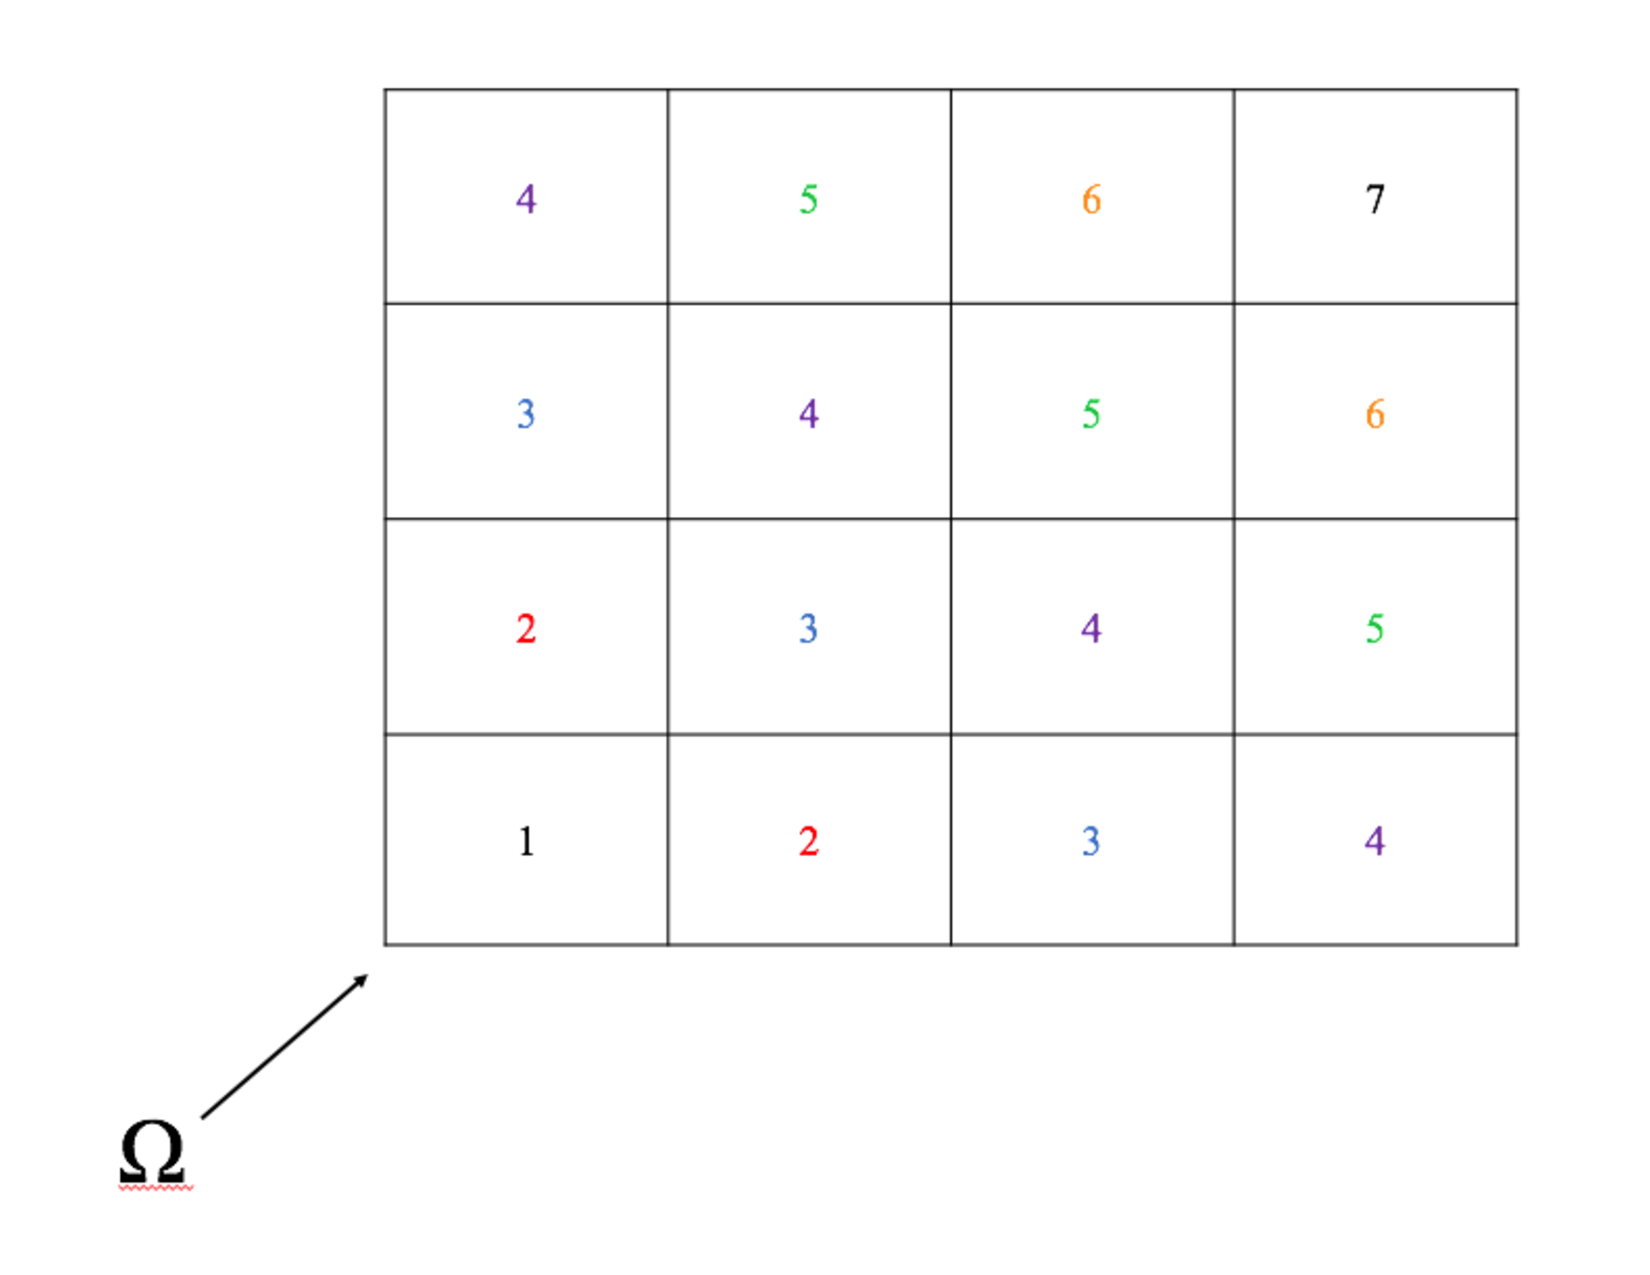
\includegraphics[scale = 0.34]{figures/StructuredMesh.pdf}
\end{frame}

\begin{frame}[t]\frametitle{Aggregation}
\begin{block}{}
		\begin{itemize}
		\item $A_x = \frac{N_x}{P_x}$, where $N_x$ is the number of cells in $x$ and $P_x$ is the number of processors in $x$
		\item $A_y = \frac{N_y}{P_y}$, where $N_y$ is the number of cells in $y$ and $P_y$ is the number of processors in $y$
		\item $N_g = \frac{G}{A_g}$
		\item $N_m = \frac{M}{A_m}$
		\item $N_k = \frac{N_z}{P_z A_z}$
		\item $N_k A_x A_y A_z = \frac{N_x N_y N_z}{P_x P_y P_z}$
		\end{itemize}
	\end{block}
\end{frame}

\begin{frame}[t]\frametitle{Parallel Efficiency}
\begin{block}{}
\begin{align*}
\epsilon &= \frac{T_{\text{task}} N_{\text{tasks}}}{[N_{\text{stages}}] [T_{\text{task}} + T_{\text{comm}}]} \\
 &=\frac{1}{[1+\frac{N_{\text{idle}}}{N_{\text{tasks}}}][1 + \frac{T_{\text{comm}}}{T_{\text{task}}}]}
\end{align*}
\end{block}
\begin{block}{}
\begin{align*}
T_{\text{comm}} &= M_L T_{\text{latency}} + T_{\text{byte}} N_{\text{bytes}} \\
T_{\text{task}} &= A_x A_y A_z A_m A_g T_{\text{grind}}
\end{align*}
\end{block}
\end{frame}

\section{Method}
\subsection{}
\begin{frame}[t]\frametitle{Metric Definitions}
	\begin{block}{}
		\begin{itemize}
			%\item We define the load balance metric, $f$.
			\item $f =\frac{\underset{ij}{\text{max}}(N_{ij})}{\frac{N_{tot}}{I\cdot J}}$
			\item $f_I = \underset{i}{\text{max}}[\sum_{j} N_{ij}]/\frac{N_{tot}}{I}$
			\item $f_J = \underset{j}{\text{max}}[\sum_{i} N_{ij}]/\frac{N_{tot}}{J}$
		\end{itemize}
	\end{block}
\end{frame}

\begin{frame}[t]\frametitle{Algorithm}
\vspace{-0.5 cm}
\begin{block}{}
\lstinputlisting[language = C++, basicstyle = \footnotesize]{loadbalance.cc}
\end{block}
\end{frame}

\begin{frame}[t]\frametitle{Redistribution}
\vspace{-0.5 cm}
\begin{block}{}
\lstinputlisting[language = C++, basicstyle = \footnotesize]{redistribute.cc}
\end{block}
\end{frame}

\section{Load Balancing Results}
\subsection{}
\begin{frame}

\end{frame}

\section{Solution Verification}
\subsection{}
\begin{frame}

\end{frame}

\section{Conclusions}
\subsection{}
\begin{frame}

\end{frame}



%\begin{frame}[allowframebreaks]{Bibliography}
%\bibliographystyle{alpha}
%\bibliography{science}
% \nocite{*}
%\end{frame}



%\section{\ }
%\begin{frame}[t]\frametitle{Sources}
%	\nocite{Dubcova20111182}
%	\nocite{CHAUVET}
%	\bibliographystyle{ieeetr}
%	\bibliography{science.bib}
%	
%	
%\end{frame}
%



\end{document}